\chapter{Metodologia Sperimentale}

\medskip

\section{Descrizione Dataset}
I dataset utilizzati nel presente lavoro di Tesi sono il risultato della ricerca dell'articolo qui citato \cite{zoppi}. Le features contenute nel dataset sono state ottenute monitorando degli indicatori di performance di un dispositivo chiamato ARANCINO \cite{arancino}, che \`e il nome commerciale per una famiglia di schede IoT e embedded che risiedono sull'omonima architettura. In istanti di tempo casuali, il dispositivo \`e stato sottoposto a delle \textit{error injections} della durata costante di 5 secondi. Gli errori con cui \`e stato attaccato il dispositivo sono di 8 tipi:

\begin{itemize}
    \item CPU usage
    \item RAM usage
    \item Deadlock
    \item Redis read
    \item Redis write
    \item Stuck arancino
    \item Stuck node-red
\end{itemize}


Gli indicatori di performance monitorati sono stati presi a livello hardware, a livello di sistema, dai sensori, dall'ambiente e a livello di applicazione. In particolare le features presenti nel dataset possono essere suddivise nelle seguenti 7 categorie:

\begin{itemize}
    \item Network: 32 features
    \item Chip Temperature: 1 feature
    \item Virtual Memory: 116 features
    \item Memory Info: 38 features
    \item IO Stats: 6 features
    \item Python Indicators: 55 features
    \item Redis DB: 25 features
\end{itemize}

Ogni osservazione \`e dotata di un'etichetta che fornisce l'informazione sullo stato del dispositivo: normale o anomalo (durante le \textit{error injections}). Se lo stato \`e normale l'etichetta corrisponder\`a a 'normal' altrimenti sar\`a una stringa che descrive l'\textit{error injection} perpetrata in quel momento nel sistema.
I dataset a disposizione sono stati:
\begin{itemize}
    \item \textit{unifi-filtered}: 69000 osservazioni. Il dispositivo \`e connesso al WiFi dell'Universit\`a degli Studi di Firenze.
    \item \textit{homenet-filtered}: 72000 osservazioni. Il dispositivo \`e connesso al WiFi di un appartamento residenziale.
    \item \textit{mobile-filtered}: 13000 osservazioni. Il dispositivo \`e connesso a una WiFi privata (ad esempio usando il tethering da una connessione mobile).
    \item \textit{all3}: 154000 osservazioni, \`e l'unione dei primi 3 dataset
\end{itemize}


\subsection{Dataset unifi-filtered}
Il dataset su cui sono stati addestrati i modelli \`e \textit{unifi-filtered}. Sono presenti 69000 osservazioni totali, di cui 11989 osservazioni etichettate come anomalie.

\begin{figure}[H]
    \centering
    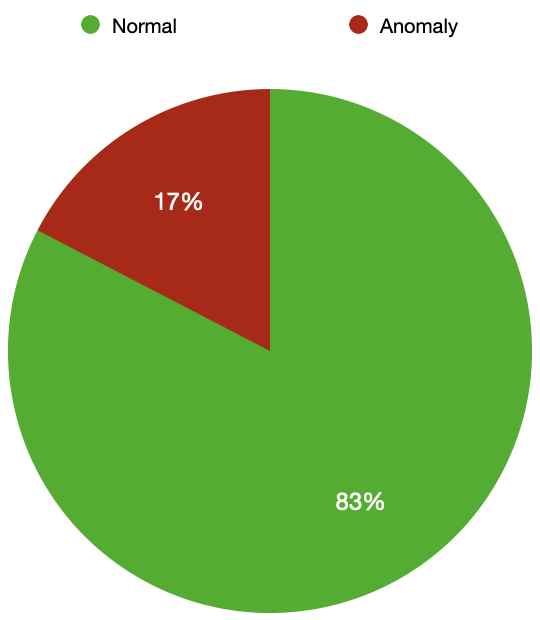
\includegraphics[width=0.5\linewidth]{balance_unifi.png}
    \caption{Composizione Dataset unifi-filtered}
    \label{fig:enter-label}
\end{figure}



\subsection{Dataset all3}
Il dataset \textit{all3} \`e stato utilizzato come test set per valutare le performance dei modelli su istanze diverse del problema. In realt\`a, non \`e stato utilizzato il dataset \textit{all3}, ma una sua versione modificata. Avendo \textit{all3} tutte le osservazioni al suo interno, comprese quelle su cui sono stati addestrati i modelli, se fosse stato utilizzato come test set avremmo testato i modelli anche su input su cui erano gi\`a stati addestrati, ottenendo come risultato delle metriche inaccurate. Per risolvere questo problema abbiamo creato una versione custom di \textit{all3} chiamata \textit{my-all3}, unendo il dataset \textit{homenet-filtered} e \textit{mobile-filtered} con solo il set di dati di test di \textit{unifi-filtered}, senza i dati di addestramento.
In \textit{my-all3} sono presenti 105700 osservazioni totali, di cui 18245 etichettate come anomalie.

\begin{figure}[H]
    \centering
    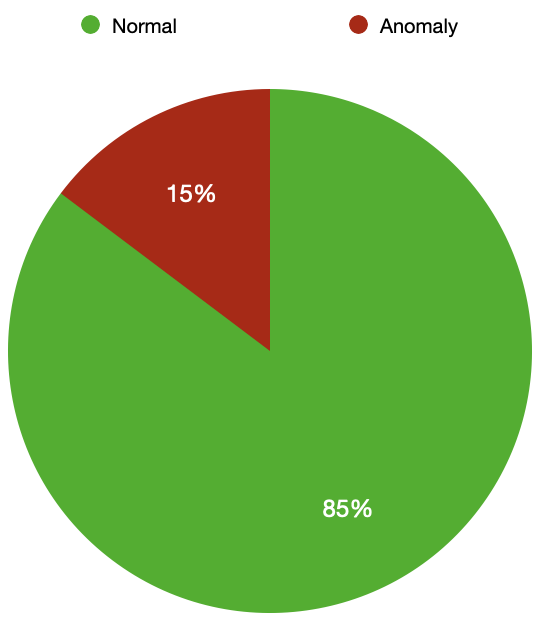
\includegraphics[width=0.5\linewidth]{balance_myall3.png}
    \caption{Composizione Dataset my-all3}
    \label{fig:enter-label}
\end{figure}



\section{Preprocessing}
I dataset utilizzati erano gi\`a stati in parte preprocessati, ad esempio non erano presenti righe con valori NaN e i dati categorici erano gi\`a stati convertiti in dati numerici.
Le operazioni di preprocessing aggiuntive sono state:

\begin{itemize}
    \item Eliminazione delle features con valori costanti. Ad esempio erano presenti features in cui il valore non variava mai e rimaneva sempre uguale a $1$, quindi non fornivano nessuna informazione utile ai modelli.
    \item Trasformazione delle etichette con la descrizione delle diverse anomalie in \textit{'anomaly'}. In questo modo \`e stato trasformato un problema di classificazione multiclasse in un problema di classificazione binaria.
    \item Mapping delle etichette da \textit{'normal'} e \textit{'anomaly'} a $0$ e $1$, rispettivamente. In questo modo anche l'etichetta \`e diventata un valore numerico e abbiamo soltanto dati numerici nel dataset.
\end{itemize}

\begin{figure}[H]
    \centering
    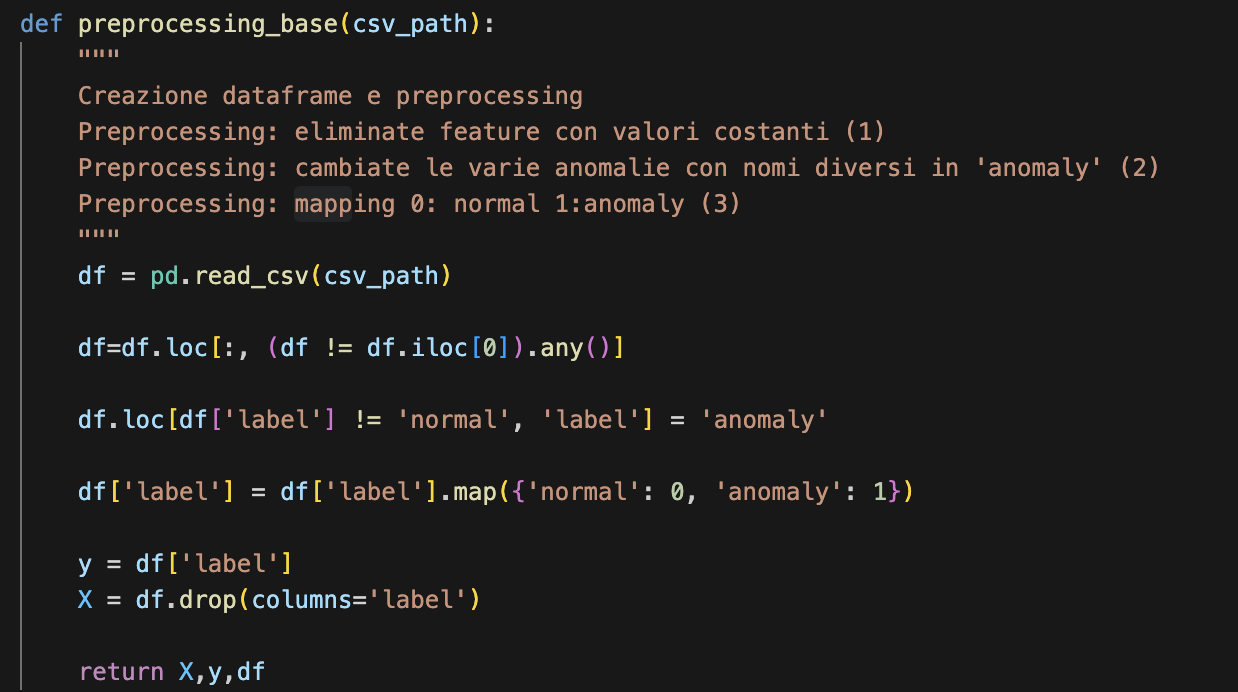
\includegraphics[width=0.9\linewidth]{preprocessing.png}
    \caption{Funzione per preprocessing datasets}
    \label{fig:enter-label}
\end{figure}

L'ultima operazione di preprocessing \`e stata standardizzare i dataset attraverso l'utilizzo della classe \textit{StandardScaler()} presente nel modulo \textit{scikit-learn}. Questa operazione di preprocessing permette di elaborare la riduzione in scala dei dati, trasformando le serie di valori in una distribuzione normale standard con media uguale a $0$ e deviazione standard uguale a $1$ \cite{stdscaler}. Standardizzare i dati \`e un'operazione di preprocessing con la quale solitamente si ottengono delle performance migliori nel processo di apprendimento.

\section{Metrica Speed Score}
Per il problema trattato in questo lavoro di Tesi \`e stato ritenuto opportuno creare una nuova metrica, chiamata \textbf{Speed Score (SS)} per misurare le performance dei modelli. Lo scopo di questa metrica \`e quello di misurare la velocit\`a con cui i modelli rilevano le anomalie. Ovviamente nell'anomaly detection \`e molto importante che le anomalie vengano rilevate nel minor tempo possibile. Per comprendere la formula del SS basta ricordare che le anomalie sono sempre presenti per 5 istanti di tempo (5 secondi), ovvero 5 righe del dataset. La formula per lo speed score \`e una somma pesata delle frequenze di rilevamento con decrescita quadratica e non lineare, per dare maggiore importanza alle rilevazioni nei primi istanti di tempo, diviso il totale delle anomalie rilevate.
  
    \begin{equation}
      SS = \frac{x_0 \cdot 1 + x_1 \cdot 0.8^2 + x_2 \cdot 0.6^2 + x_3 \cdot 0.4^2 + x_4 \cdot 0.2^2}{TotaleAnomalie}
    \end{equation}

    Con $x_0, x_1, x_2, x_3, x_4$ che indicano rispettivamente il numero di anomalie rilevata al primo, secondo, terzo, quarto e quinto istante di tempo.

\section{Strategie}
Le strategie adottate per l'addestramento dei modelli sono state 3 in totale. Un approccio classico, senza alcuna modifica al dataset \textit{unifi-filtered}, e 2 approcci time series, intervenendo sulla struttura del dataset. Entrambi gli approcci time series sono stati ottenuti andando a modificare i dataset, aggiungendo delle nuove features che portassero dell'informazione time series con loro. In generale per ogni modello \`e stato calcolato l'MCC, lo speed score e infine l'accuracy tramite cross-validation. Inoltre \`e stata graficata per tutti i modelli la progressione delle metriche appena menzionate rispetto agli approcci utilizzati. \`E stato graficato anche un confronto tra la progressione dei valori di MCC calcolati sul test set di \textit{unifi-filtered} e quella su \textit{my-all3}.

\subsection{Approccio Classico}
Nell'approccio classico \`e stato effettuato il training dei 4 modelli, che ricordiamo essere Logistic Regression, Linear Discriminant Analysis, Random Forest e XGBoost, sul dataset \textit{unifi-filtered} senza alcuna modifica, a parte le operazioni di preprocessing.

\subsection{Approccio Time Series con Media Mobile}
La media mobile semplice (SMA, \textit{simple moving average}) \`e un indicatore molto utilizzato nell'analisi di serie storiche, questo perch\'e ogni punto della media mobile porta con s\'e l'informazione di $n$ istanti di tempo precedenti. Diamo la definizione di media mobile semplice: data una serie storica $y_t$ con $t=1,2,...T$ contenente i valori osservati di una variabile $Y$ dal tempo 1 al tempo $T$ si definisce media mobile al tempo $t$ il valore \cite{sma}:

  \begin{equation}
      SMA=\frac{1}{k} \sum_{i=t-k+1}^{t} y_{i} \hspace{1cm} \text{con $t \geq k$}
  \end{equation} 
dove $k$ \`e il periodo della media mobile, ed equivale al numero degli addendi.

Il primo approccio sperimentato \`e stato quello di creare per ogni feature presente nel dataset una feature aggiuntiva che contenesse il valore della media mobile semplice (SMA) di $n$ istanti precedenti. In questo modo i modelli sono stati addestrati sul doppio delle features, dato che per ogni \textit{feature} \`e stata creata la corrispondente feature \textit{feature-media-mobile}, con a disposizione le importanti informazioni su come i valori delle features siano evoluti nel tempo. 

\begin{figure}[H]
    \centering
    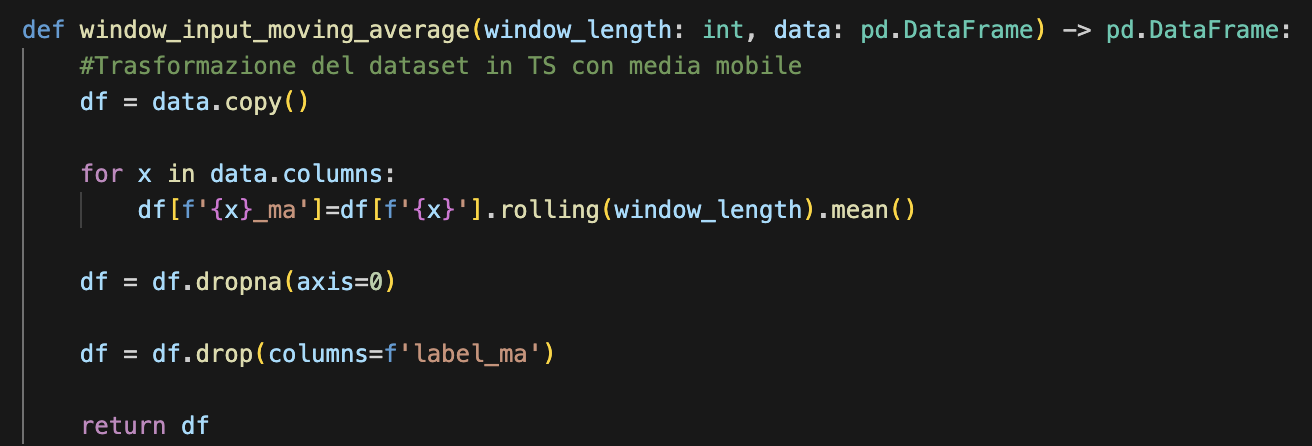
\includegraphics[width=0.9\linewidth]{def_ts_ma.png}
    \caption{Funzione per trasformazione dataset con features media mobile}
    \label{fig:enter-label}
\end{figure}

 
\subsection{Approccio Time Series con Differenze}
Un altro modo di portare informazioni time series all'interno del dataset \`e stato quello di aggiungere delle nuove features che contenessero la differenza tra il valore attuale delle features e il loro valore precedente. Anche in questo caso, come per la media mobile, le differenze sono state calcolate su $n$ istanti di tempo, quindi per ogni feature sono presenti altre $n$ features che rappresentano la differenza tra il valore attuale all'istante $t$ e i valori all'istante $t-1,t-2,...t-n$.

\begin{figure}[H]
    \centering
    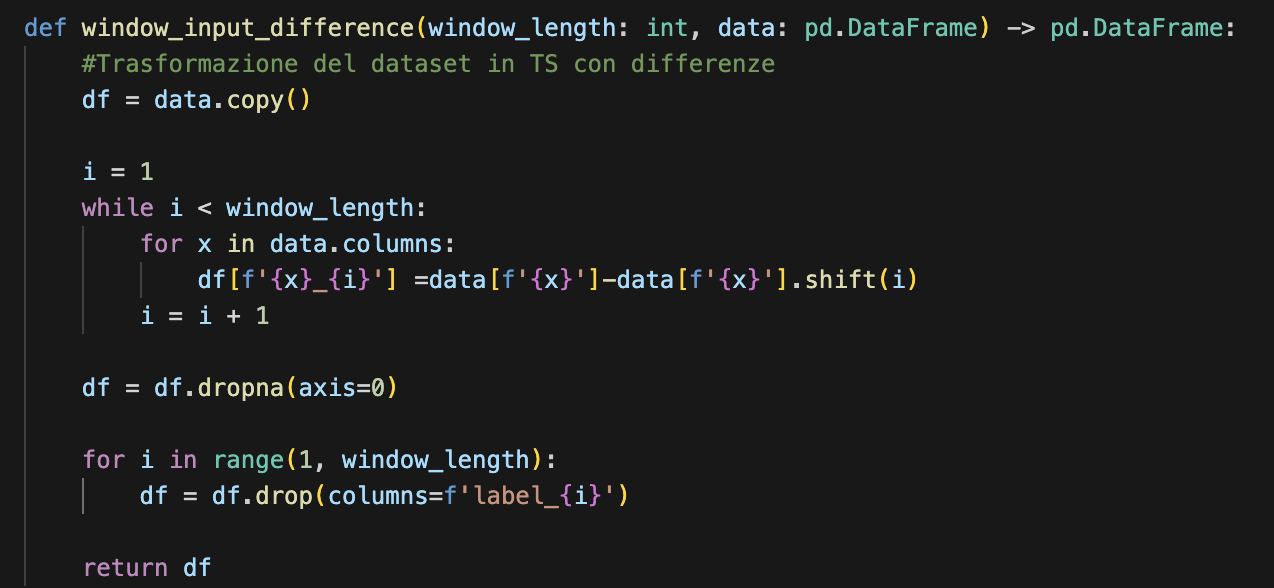
\includegraphics[width=0.9\linewidth]{def_ts_diff.png}
    \caption{Funzione per trasformazione dataset con features differenze}
    \label{fig:enter-label}
\end{figure}

\section{Window e Shuffle}
Gli approcci finora descritti sono stati valutati sulla base di due parametri molto importanti: \textit{window} (nel codice \textit{window\_length}) e \textit{shuffle}. \textit{Window} \`e il nome dato al parametro che definisce la finestra temporale, ovvero il numero di istanti di tempo, su cui vengono calcolate la media mobile e le differenze negli approcci time series. La funzione \textit{train\_test\_split} \`e stata utilizzata per dividere il dataset in set di training e set di test e il parametro \textit{shuffle} \`e un parametro booleano che stabilisce se rimescolare o meno i dati prima della suddivisione in train set e test set \cite{train_test_split}.

\subsection{Window}
Negli approcci time series sono stati utilizzati diversi valori per il parametro \textit{window} e quindi per la finestra temporale. Per i valori da assegnare a \textit{window} \`e stato scelto un intervallo $[2,5]$. Per chiarezza, con $window=2$ nel caso delle differenze viene aggiunta al dataset 1 feature per ogni feature presente con la differenza tra il valore all'istante $t$ e il valore all'istante $t-1$, mentre nel caso della media mobile la media sar\`a calcolata tra i valori agli istanti di tempo $t$ e $t-1$. Con $window=5$ nel caso delle differenze verranno aggiunte al dataset 4 features per ogni feature presente con le differenze tra il valore all'istante $t$ e il valore gli istanti $t-1,t-2,t-3,t-4$, mentre per la media mobile la media sar\`a calcolata tra i valori agli istanti $t,t-1,t-2,t-3,t-4$.
L'intervallo $[2,5]$ \`e stato scelto perch\'e 2 rappresenta la finestra temporale minima e 5 \`e il numero di secondi per cui le anomalie si protraggono all'interno del sistema.
Lo scopo \`e stato quello di verificare come le performance dei modelli andassero a cambiare al variare della finestra temporale.

\subsection{Shuffle}
In generale non \`e appropriato rimescolare i dati quando si tratta di dati time series. Questo perch\'e ci\`o che contraddistingue i dati time series dagli altri tipi di dati, \`e che i dati sono raccolti nel tempo e c'\`e correlazione tra osservazioni adiacenti, quindi preservare l'ordine dei dati \`e importante. Per questo di default durante i vari training dei modelli il parametro \textit{shuffle} \`e sempre stato impostato a \textit{False}. Abbiamo comunque voluto verificare quali fossero le differenze di performance dei modelli con il parametro $shuffle=True$. Da notare che con un valore diverso di \textit{shuffle} cambiano i dati nel set di training del modello e quindi si hanno performance e feature importance diverse.

 \vspace{-0.5cm}
 \vspace{-0.3cm}